The AEON platform (see Vision) provides a modular environment of mechatronic elements, monitoring and recording pathways, and data curation tools, enabling continuous high-resolution behavioural and neural measurement over an unprecedented timescale of many weeks to months.  To fully realise the scientific potential of the Naturalistic Long-Duration and Continual (NaLoDuCo) data created by AEON and similar platforms, we plan to develop complementary open-source software frameworks for (offline) data analysis, visualisation and (online) real-time processing including for spike-sorting.

\subsubsection{Offline analysis methods}
\label{sec:offlineAnalysisMethods}

\input{offlineMethods}

\subsubsection{Real-time machine learning methods}
\label{sec:rtmlMethods}

Real-time machine learning (RTML) remains underutilised in neuroscience. This represents a missed opportunity—especially in the context of NaLoDuCo experimentation—where adaptive, low-latency computation could greatly enhance experimental control and scientific discovery.

We will attempt a real time implementation of the pipeline in Table 1, adapted for robustness in non-stationary evironments.

\subsubsubsection{Bonsai and Bonsai.ML}

Bonsai is a widely adopted open-source software ecosystem for experimental
control in neuroscience~\cite{lopesEtAl15}. With support from the
\href{https://gow.bbsrc.ukri.org/grants/AwardDetails.aspx?FundingReference=BB\%2FW019132\%2F1}{BBSRC},
we are developing infrastructure for intelligent, closed-loop experimentation
through the \href{https://bonsai-rx.org/machinelearning/}{Bonsai.ML} package.

We have already integrated several real-time ML models into Bonsai.ML,
including linear regression, linear dynamical systems, hidden Markov models,
and Bayesian point-process decoders. In collaboration with researchers at SWC
and UCL, we are applying these models to real-time inference of visual
receptive fields, foraging kinematics, behavioural state classification, and
spatial decoding of hippocampal spiking activity (see the
\href{https://bonsai-rx.org/machinelearning/examples/README.html}{Bonsai.ML examples}).

However, current Bonsai.ML models assume stationarity—a strong and often
invalid assumption in NaLoDuCo contexts. We will adapt these methods to operate
under non-stationary conditions using the previously described techniques.

Linear models from adaptive signal processing, such as least mean squares and
recursive least squares, are already suited for real-time use and require no
major modification. Nonlinear regression, particularly using artificial neural
networks (ANNs), can support real-time inference (especially on GPUs), but
real-time learning is more challenging. Continual learning methods—such as
experience replay and online regularization—introduce additional computational
overhead (e.g., data buffering, importance weight tracking) that may exceed the
constraints of real-time systems. To address these constraints, we will explore
adaptation strategies:

\begin{enumerate}

	\item\textbf{Real-time minibatch updates:} Training is performed on small
	minibatches as data arrive, balancing learning speed with latency.

	\item\textbf{Bounded-time updates:} Only a subset of model parameters
	(e.g., output layer weights) is updated to reduce computation time.

	\item\textbf{Hybrid strategy:} A dual-pipeline system in which a
	lightweight process performs fast inference, while a slower process
	(running on a separate processor or node) accumulates recent data in a
	rolling buffer and periodically retrains or updates the model. The updated
	model is deployed into the fast path only after validation, ensuring
	continuity in inference.

\end{enumerate}

All new RTML tools will be released as open-source extensions to the
\href{https://bonsai-rx.org/machinelearning/}{Bonsai.ML} package.

\subsubsubsection{Experimental Replays in AEON}

We will extend the AEON platform with functionality to replay previously
recorded experimental data. Real-time machine learning (RTML) objects in AEON
typically receive input from live data streams—such as video frames from
cameras or voltage measurements from Neuropixels probes—each precisely
timestamped using the HARP protocol. This protocol ensures that every item in
the stream is tagged with the exact time it occurred during the experiment.

The new replay feature will regenerate all data streams from a previous
experiment and deliver each data item to its observers at exactly the same
relative time as in the original experiment. This enables RTML components to be
tested under identical conditions to those in live experiments, while
eliminating the need to rerun time-consuming and resource-intensive
experiments. This supports the 3Rs by reducing animal use (Reduction) and
enabling partial replacement of live testing (Replacement).

Replay functionality will enable comprehensive testing of RTML methods.
Researchers will be able to debug their pipelines, evaluate different parameter
settings, and verify that real-time constraints are met—all without placing
additional demands on experimental animals or facilities. This is particularly
critical in NaLoDuCo settings, where experiments run continuously for weeks or
months and are costly, laborious, and ethically sensitive.

\subsubsubsection{Deliverables}

\begin{enumerate}

	\item New real-time machine learning methods for non-stationary
	experimental control, integrated into the open-source
	\href{https://bonsai-rx.org/machinelearning/}{Bonsai.ML} package.

	\item AEON experimental replay functionality enabling real-time
	reproductions of previously recorded AEON experiments, saving time,
	resources and animal experiments.

	\item Peer-reviewed publications co-authored with SWC and AIND researchers,
	showcasing scientific advances made possible by the new RTML capabilities.

\end{enumerate}


\subsubsection{Visual exploration}
\label{sec:visualExploration}

Visualisations are essential for extracting insight from any dataset. Given the
scale of NaLoDuCo datasets, downloading them locally is impractical. Therefore,
visualisation methods must operate where the data resides—either in the cloud
or on institutional HPC systems.

We will develop visualisation functionality for both continuous datasets and
epoched datasets, where epochs are anchored around events identified by
advanced machine learning methods.

\subsubsubsection{Continuous visualisations}

Continuous visualizations will allow users to intuitively explore large-scale
behavioral and neural datasets spanning weeks to months. Users will be able to
zoom out for a high-level overview (e.g., a full month) or zoom in to examine
millisecond-level details, offering an interactive experience similar to Google
Maps for time series data.

To enable this, we will implement:

\begin{itemize}

	\item\textbf{Multi-Resolution Tiling:} Datasets will be preprocessed into
	tiles at various spatial and temporal resolutions, rendering only relevant
	tiles as users zoom.

	\item\textbf{Hierarchical Storage:} Data will be organized using formats
	such as Zarr or HDF5 to support chunked, multi-resolution access.

	\item\textbf{On-Demand Streaming:} Visualizations will stream data
	dynamically, adapting to the user's current view.

\end{itemize}

\subsubsubsection{Epoched and interactive visual analytics}

A key strength of our platform is its support for epoched visualisation and
interactive, closed-loop visual analytics, which together enable the discovery
and refinement of neural and behavioural patterns in long-duration datasets.

\paragraph{Machine Learning-Defined Events.} A core feature of our system will
be the ability to align epochs not just to experimenter-defined events, but
also to latent state transitions inferred via unsupervised methods (e.g.,
hidden Markov models, behavioural clustering, inverse reinforcement learning)

\paragraph{Closed-Loop Analytics.} There will be a closed-loop interaction
between visualisations and machine learning algorithms. In this loop:

\begin{itemize}

	\item \textbf{Machine learning algorithms} extract latent states, classify
	behaviours, infer structure, or forecast dynamics from NaLoDuCo data.

	\item These outputs feed into the visualisation engine to generate novel
	views (e.g., state-aligned rasters, dynamic embeddings, attention maps).

	\item \textbf{Users explore these visualisations interactively},
	discovering unexpected, task-agnostic, or contextual patterns.

	\item New queries and insights drive further rounds of machine learning
	analysis—closing the loop.

\end{itemize}

This design enables researchers to co-develop computational models and
scientific hypotheses iteratively, with human insight and machine inference
deeply intertwined.

\subsubsubsection{Deliverables}

\begin{enumerate}

	\item visualisations for continuous behavioural and neural recording

	\item visualisations for epoched behavioural and neural recording

	\item visualisations for model outputs

	\item indexing system to support intelligent visualisations

	\item deployment of the above items to allow users to visualise NaLoDuCo
	DANDI datasets on the cloud

\end{enumerate}


\subsubsection{Offline spike sorting}
\label{sec:offlineSpikeSorting}

Extracting single-unit activity from raw, long-duration extracellular
recordings presents major challenges. Continuous neural recordings over weeks
or months, as in NaLoDuCo experiments, exhibit complex non-stationarities in
signal properties and produce massive datasets—often hundreds of terabytes in
size. These characteristics break many assumptions underlying conventional
spike sorting approaches and make manual curation infeasible.

To address these challenges our approach integrates experimental and
computational strategies. Experimentally, we will minimise electrode-tissue
movement by cementing probes to the skull, as in~\cite{schoonoverEtAl21}.
Computationally, we will create spike sorting strategies addressing
non-stationarities in NaLoDuCo recordings, distribute computation across
multiple nodes and use GPU acceleration to manage scale, and create automatic
curation methods tailored to non-stationarities in NaLoDuCo experimentation.

\subsubsubsection{Spike sorting approach for long-duration NaLoDuCo recordings}

In order to perform spike sorting on long-duration datasets, we will use an
overlapping windowing approach. Spike sorting will be done in short-duration
windows of a few hours (e.g., five hours), with a partial overlap between
consecutive windows (e.g., one hour).  We will first run spike sorting (e.g.,
Kilosort4) independently for each window. Next, we will use the overlapping
segment to compare the spike trains extracted from the two consecutive windows,
using existing methods implemented in SpikeInterface~\cite{buccinoEtAl20}. Assuming that
the spike sorter will find the same units and (most of) their spikes in that
period, unit identities will be tracked by finding the unit pairs on
consecutive sessions with the highest spike-train agreement in the overlapping
interval (we refer to this as consecutive tracking).

\subsubsubsection{Automatic quality control}

The long-duration of NaLoDuCo recordings and the large number of individual
spike sorting jobs makes manual inspection and curation unfeasible. We will
therefore integrate and evaluate the performance of two recently developed
automated tools to label spike sorted units: Bombcell\cite{fabreEtAl23} and
UnitRefine\cite{jainEtAl25}.  Both tools assign quality labels to individual
units (“good,” “multiunit activity” or “noise”)

After evaluating and fine-tuning the performance of Bombcell and UnitRefine on
individual spike sorting outputs, we will run automatic quality control
separately for each short-window spike sorting output. Using the new
visualisations we will develop, researchers will be able to explore quality
trends over timescales ranging from hours to weeks, detect periods of
instability, and automatically flag clusters exhibiting inconsistent or
transient quality metrics.

\subsubsubsection{Long-term tracking of units}

The extended duration of NaLoDuCo recordings introduces various forms of
non-stationarity, including tissue–electrode interactions, probe degradation,
neural plasticity, and brain state fluctuations. These factors can alter
neuronal waveforms over time and complicate spike sorting. To address this, we
will complement local unit tracking with long-term global tracking by extending
methods such as UnitMatch~\cite{vanBeestEtAl24} or the earth-moving-distance-based
approach~\cite{yuanEtAl24}. These extensions will maintain a catalogue of all
detected units, enabling reconciliation of unit identities across epochs where
waveforms shift or units transiently disappear.

\subsubsubsection{Spike sorting on the cloud/institutional HPC systems}

The very large size of NaLoDuCo recordings requires running spike sorting where
the data resides. We will build a web-based application to launch scalable
spike sorting jobs on multiple backends, including cloud providers and HPC
systems, and to visualise spike sorting results.

To run spike sorting at scale, we will extend an
\href{https://github.com/AllenNeuralDynamics/aind-ephys-pipeline}{existing
pipeline developed at AIND for spike sorting of Neuropixels data}. The pipeline
will be adapted for long-duration NaLoDuCo recordings to massively parallelize
all spike sorting jobs of short-duration windows, to automatically curate their
spike sorting results, to collect and compare the overlapping windows to track
unit identities, and to track long-term identities.

To visualise spike sorting results over extended periods will use the methods
described in Section Visual Exploration.

\subsubsubsection{Deliverables}

\begin{enumerate}

	\item Development of a spike sorting strategy for high-channel-count and long-duration recordings.

	\item Automated unit tracking and quality control across extended recordings.

	\item Web-based application to launch spike-sorting jobs on remote servers and to visualise long-duration spike sorting results.

	\item Spike sorting pipeline for cloud/HPC deployments for scalable and reproducible processing.

	\item Open-source release of all spike sorting tools, quality metrics, cloud deployment scripts, and documentation.

\end{enumerate}



\subsubsection{Online spike sorting}
\label{sec:onlineSpikeSorting}

Few methods currently support online spike sorting for high-channel-count
probes. To the best of our knowledge, there is currently no readily-usable
online spike sorting solution available for chronic Neuropixels recordings in
freely moving mice.

We will implement a new online and adaptive spike-sorting method using the
hybrid strategy described in Section~Bonsai and Bonsai.ML.
%
Periodically, as new chunks of recording become available, the slower process
in this strategy will update a catalogue of waveforms of detected units, as
indicated in Section~Offline Spike Sorting.
%
With this catalogue, the lightweight process will perform template matching
(i.e., detect spikes and match the corresponding waveform to that of a unit in
the catalogue).
%
It will implemented as a Bonsai observable, and will operate on short chunks
of tens to hundreds of milliseconds.
%
Since several template matching algorithms are available, we will benchmark
them in terms of speed and accuracy against the offline spike sorting results.

As online spike sorting will become essential for future adaptive experiments,
we will integrate our solution into SWC and AIND Bonsai workflows for
real-time visualization and spike-based analysis.

\subsubsubsection{Deliverables}

\begin{enumerate}

    \item A new online spike-sorting method robust to non-stationarities in
        NaLoDuCo experimentation, targeting a latency in the order of tens to
        hundreds of milliseconds.

    \item Integration of the new online spike sorting method into existing
        Bonsai workflows at the SWC and AIND for closed-loop control and
        real-time experimental feedback.

    \item Open-source dissemination of code and tools for real-time spike
        sorting, including documentation and example Bonsai workflows using
        NaLoDuCo data.

\end{enumerate}



\subsubsection{Project management}
\label{sec:projectMgmt}


\begin{figure}
    \begin{center}
        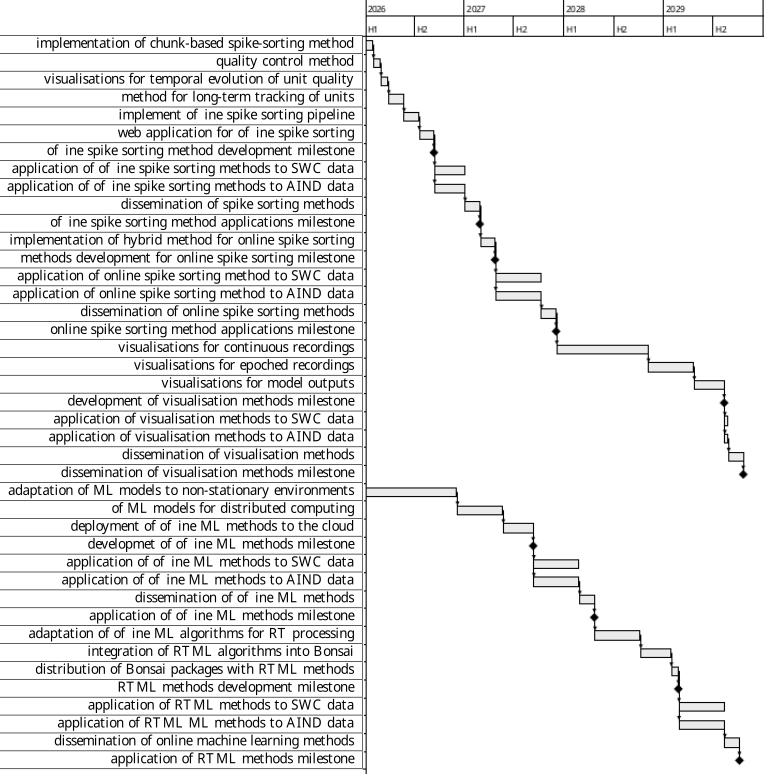
\includegraphics[width=5in]{figures/bbsrc-nsfbio24_gantt.png}
        \caption{gantt chart}
        \label{fig:ganttChart}
    \end{center}
\end{figure}




